\section{Versuchsaufbau}
\label{sec:Versuchaufbau}
\begin{figure}
    \centering
    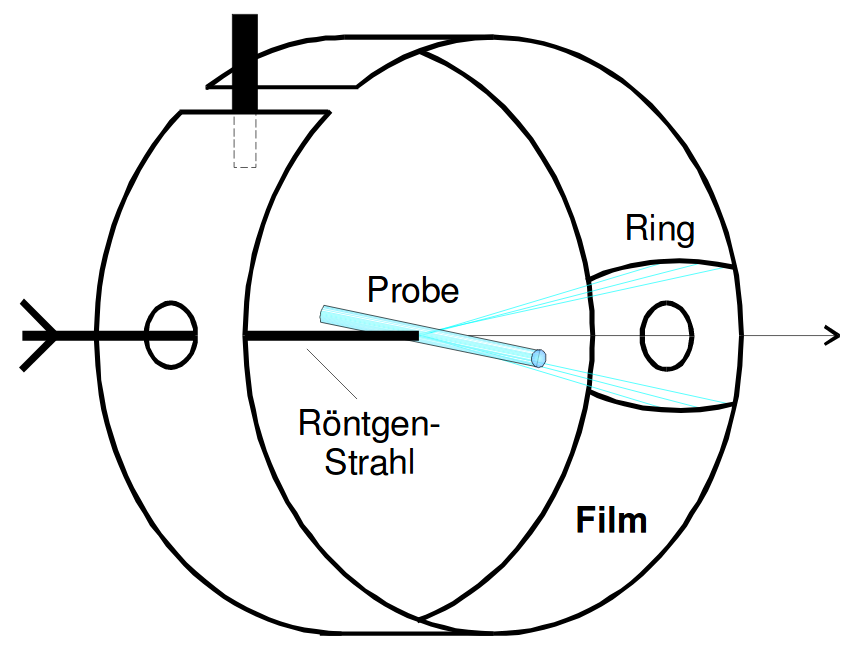
\includegraphics[width=0.55\textwidth]{ressources/aufbau.png}
    \caption{Skizzenhafter Aufbau zu Aufnahme der Filme mittels Debye-Scherrer Methode\cite{skript}.}
    \label{aufbau}
\end{figure}
Mithilfe des Debye-Scherrer-Verfahrens wird experimentell die Struktur eines
Kristalls bestimmt. Der zylindrische Stab, welcher mit einer pulverisierten
Probe gleichmäßig beschichtet ist, wird mittig mit monochromatischen
Röntgenstrahlen belichtet. Während der Bestrahlung setzt ein Motor die Probe in
ihrer Längsachse in Rotation. Bei der Belichtung ist es äußerst wahrscheinlich,
dass sich einige Kristalle in der Reflexionsstellung befinden, weil die Probe in
 pulverisierter, kristalliner Form vorliegt ist die Ausrichtung der Kristallpartikel
 über den gesamten Raumwinkel verteilt. Die monochromatische Röntgenstrahlung trifft
 auf die zylindrische angeordnete Probe und wird durch verschiedene
 Netzebenenscharen {h,k,l} um einen Winkel $\theta$ abgelenkt. Der Filmstreifen hinter dem
 zylindrischen Stab dient zum Nachweis der gebeugten Röntgenstrahlen. Die Probe
 rotiert, um eine bessere Mittelung aller Reflexionen zu erhalten.
